% Chapter 7, Section 4

\section{Dropout}
\label{sec:dropout}

\textbf{Dropout} randomly deactivates neurons during training, preventing co-adaptation.

\subsection{Intuition: Training a Robust Ensemble}

Dropout is like asking different subsets of a team to work on the same task on different days. No single member can rely on a particular colleague always being present, so each learns to be broadly useful. This results in a robust team (model) that performs well even when some members (neurons) are inactive.

\subsection{Training with Dropout}

At each training step, for each layer:
\begin{enumerate}
    \item Sample binary mask $\vect{m}$ with $P(m_i = 1) = p$
    \item Apply mask: $\vect{h} = \vect{m} \odot \vect{h}$
\end{enumerate}

Mathematically:
\begin{equation}
\vect{h}_{\text{dropout}} = \vect{m} \odot f(\mat{W}\vect{x} + \vect{b})
\end{equation}

where $m_i \sim \text{Bernoulli}(p)$.

\subsection{Inference}

At test time, scale outputs by dropout probability:
\begin{equation}
\vect{h}_{\text{test}} = p \cdot f(\mat{W}\vect{x} + \vect{b})
\end{equation}

Or equivalently, scale weights during training by $\frac{1}{p}$ (inverted dropout).

\subsection{Interpretation}

Dropout can be viewed as:
\begin{itemize}
    \item Training an ensemble of $2^n$ subnetworks
    \item Adding noise to hidden activations
    \item Approximate Bayesian inference
\end{itemize}

\subsection{Variants}

\textbf{DropConnect:} drop weights instead of activations

\textbf{Spatial Dropout:} drop entire feature maps in CNNs

\textbf{Variational Dropout:} use same mask across time steps in RNNs

\begin{figure}[htbp]
\centering
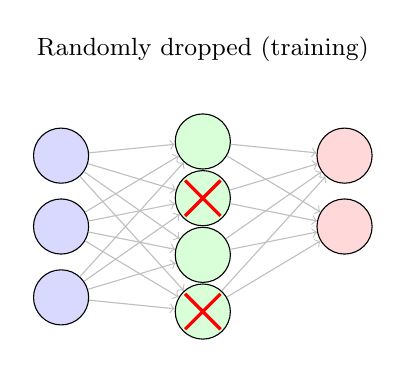
\begin{tikzpicture}[scale=0.9]
    % Layer nodes
    \foreach \i in {1,2,3}
        \node[circle, draw, fill=blue!15, minimum size=0.7cm] (x\i) at (0,-\i) {};
    \foreach \i in {1,2,3,4}
        \node[circle, draw, fill=green!15, minimum size=0.7cm] (h\i) at (2,-\i*0.8) {};
    \foreach \i in {1,2}
        \node[circle, draw, fill=red!15, minimum size=0.7cm] (y\i) at (4,-\i) {};

    % Full connections (light gray)
    \foreach \i in {1,2,3}
        \foreach \j in {1,2,3,4}
            \draw[->,gray!50] (x\i) -- (h\j);
    \foreach \i in {1,2,3,4}
        \foreach \j in {1,2}
            \draw[->,gray!50] (h\i) -- (y\j);

    % Dropped neurons (crossed)
    \draw[red, line width=1.2pt] (h2) ++(-0.25,-0.25) -- ++(0.5,0.5);
    \draw[red, line width=1.2pt] (h2) ++(0.25,-0.25) -- ++(-0.5,0.5);
    \draw[red, line width=1.2pt] (h4) ++(-0.25,-0.25) -- ++(0.5,0.5);
    \draw[red, line width=1.2pt] (h4) ++(0.25,-0.25) -- ++(-0.5,0.5);

    \node at (2,0.5) {\small Randomly dropped (training)};
\end{tikzpicture}
\caption{Dropout during training: randomly deactivating hidden units encourages redundancy and robustness.}
\label{fig:dropout-diagram}
\end{figure}

% Index entries
\index{dropout}
\index{regularization!dropout}

